The following section provides details in the construction of the model for predicting stock prices, as well as a breakdown of the data used in the training of the network.

\section{Dataset}
The data consist of daily values for NYSE listed companies for the period January 1, 2018 to December 1, 2018. The dataset includes daily information for the \texttt{close}, \texttt{open}, \texttt{high}, \texttt{low} prices and \texttt{volume} of each trading day. 


The data comprise of companies from various sectors listed in the New York Stock Exchange.

\section{Prediction Model}

Here is a sentence, and you can see a nice picture in Figure \ref{fig:brayford}.

\begin{figure}[h]
    \centering
    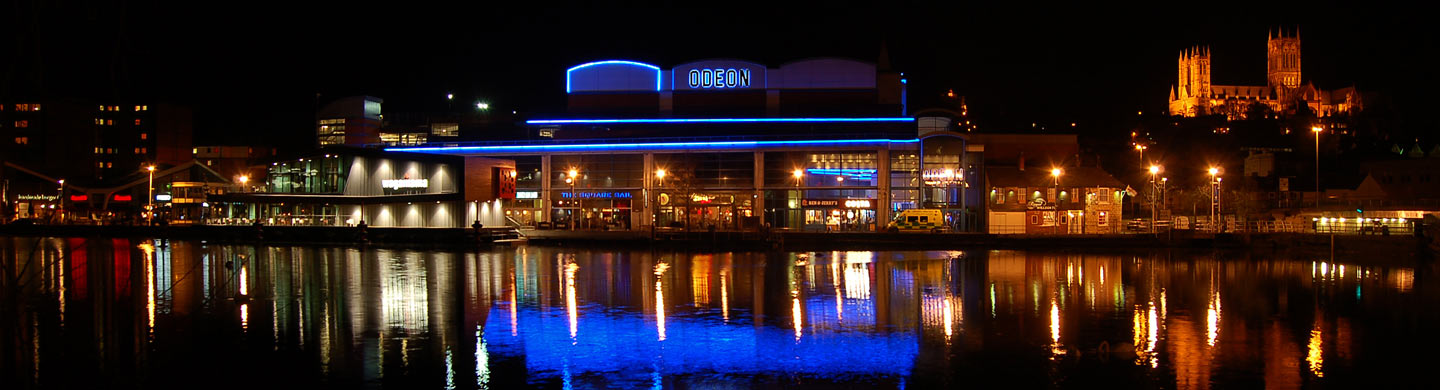
\includegraphics[width=\textwidth]{figures/brayford.jpg}
    \caption{A picture of the Brayford from Google Images.}
    \label{fig:brayford}
\end{figure}

Also, a table can be found in Table \ref{tbl:example-table}. You should use a \LaTeX~table generator like \url{https://www.tablesgenerator.com/} if you want to make your life easier.

\begin{table}[h]
    \caption{Here is a table. The caption goes above like this.}
    \centering
    \begin{tabular}{l|l|c}
        First name & Last name & Age \\
        \hline\hline
        Bob & Bobbington & 24 \\
        Joe & Bloggs & 37 \\
        Billy & Bob & 10 \\

    \end{tabular}
    \label{tbl:example-table}
\end{table}